\chapter{Validación de la solución}
\label{ch:validacion}
\section{Diseño de los contrastes}
La validación examina la correctitud de los volúmenes reconstruidos y la aplicación del mismo procedimiento en los cinco patrones. El diseño sigue el enfoque de \citet{jain1991} para definir la pregunta, la carga, los factores, las respuestas y los controles. La agrupación se estudia mediante tres mecanismos: eliminar reenvíos entre etapas, reutilizar un archivo entre consumidores y reunir tareas que consumen particiones distintas. Se examina cuándo DME aumenta, cuándo permanece constante y qué entregas explican el resultado. Los contrastes de tamaño y ubicación permiten precisar la interpretación de la referencia.

El bloque A histórico reúne 24 condiciones de la evaluación de DME con flujos sintéticos bajo CondorIO. Sus 72 ejecuciones elegibles corresponden a tres repeticiones por condición, enviadas en orden fijo. La unidad de observación es una ejecución completa. La selección posterior de quince condiciones y 45 ejecuciones organiza siete contrastes en los cinco patrones. AC1, AC2 y AC4 designan los niveles de uno, dos y cuatro consumidores por job en el caso de archivo compartido. El paquete histórico conserva sus identificadores originales; aquí se usan AC1, AC2 y AC4. R01-E y R02-E conservan sus identificadores históricos dentro del bloque A.

\subsection{Decisiones del diseño según Jain}
\label{sec:jain_diseno}
El enfoque de \citet{jain1991} y su material docente \citep{jain2017} orientan la definición del sistema, la carga, las respuestas, los factores y los controles. El servicio del sistema es ejecutar un grafo y entregar sus resultados declarados. Se usan cinco patrones con archivos de tamaños e identidades conocidos. En distribución se distinguen particiones diferentes y consumidores de un mismo archivo. Las respuestas principales son los volúmenes en bytes, DME y los conteos. La duración del flujo y los tiempos posteriores se miden por separado.

Cada contraste tiene una línea base y varía el tamaño, la agrupación o la ubicación según la pregunta. Se conserva el resto de los controles pertinentes y se verifica su valor efectivo con el plan y el historial. Los niveles de las fichas explican qué cambia y por qué. Los contrastes permiten comprobar el cálculo por archivo y destino. Un diseño factorial permitiría examinar interacciones entre los factores con niveles comparables en todos los patrones. El requerido se deriva de la definición; las cuentas del observado se reconstruyeron retrospectivamente desde contratos preservados y no constituyen predicciones previas al experimento.

\subsection*{Cobertura de la selección}
La Tabla~\ref{tab:fuera_contrastes} identifica las nueve condiciones elegibles que quedaron fuera de las fichas. La selección retrospectiva permite comprobar las cuentas de cada contraste. Estimar la frecuencia de estos comportamientos en otros flujos requeriría otro diseño. Las otras condiciones documentan asignaciones alternativas, cambios en el número de tareas, un nivel adicional de agrupación o cambios de pool y ubicación. Sus 27 ejecuciones se conservan como archivo de campaña y no integran las tablas de DME de esta tesis. El cotejo detallado de 348 direcciones de este capítulo corresponde a las 45 ejecuciones seleccionadas.

\begin{table}[htbp]\centering\small
\caption{Condiciones elegibles fuera de las fichas de validación}
\label{tab:fuera_contrastes}
\begin{tabularx}{\linewidth}{@{}P{3.3cm}Y@{}}
\toprule Condiciones & Qué añaden al bloque A\\\midrule
L02, D01 & Asignaciones alternativas del pipeline y de distribución.\\
L05 & Pipeline más largo, de cinco etapas.\\
A02B, D02B, R02B & Grafos de agregación, distribución y redistribución con menos ramas.\\
GD2 & Nivel intermedio entre D02 y GD4 para agrupar particiones distintas.\\
W01, W04 & Cambios conjuntos de asignación y número de máquinas disponibles.\\
\bottomrule
\end{tabularx}
\end{table}


\subsection{Líneas base y controles comunes}
La línea base es la configuración ejecutada con la cual se compara una variante. El volumen requerido se calcula por separado para cada ejecución. La sección~\ref{sec:repro_patrones} identifica las bases y variantes de los siete contrastes, con su justificación, cuenta esperada y decisión respaldada por los datos.



Los 10 MiB permiten seguir las entregas del pipeline. En procesamiento se duplica ese tamaño a 20 MiB. En I40 se cambia solo un intermedio a 40 MiB. Estos niveles sirven para comprobar cambios de volumen en cargas controladas. El tiempo se mide por separado.

En los contrastes históricos de agrupación se conservan el grafo, los tamaños, la asignación y la política de entrega. En los de ubicación se mantienen los archivos y la organización en jobs. R02-E modifica la asignación de varias etapas a la vez. Su efecto sobre el requerido se desglosa por dependencia, mientras que la duración corresponde a la configuración completa.

\subsection{Entorno y orden de toma de datos}
El bloque A se ejecutó con Pegasus 5.1.2, HTCondor 26.0.1 (compilación DAILY) y CondorIO en máquinas virtuales Ubuntu Server 24.04 LTS x64, en una misma región de la nube. Los manuales citados describen Pegasus 5.1.3. Los contratos se verificaron con los planes y registros de 5.1.2; no se presupone equivalencia entre versiones ni estabilidad fuera de la compilación ensayada. L01-r01 se excluyó por un cambio de intervalos durante la ejecución (sección~\ref{sec:protocolo_a}). El coordinador tiene dos CPU virtuales y cerca de 6,77 GiB visibles. Cada worker tiene una CPU virtual y cerca de 3,33 GiB visibles. El slot anuncia una CPU y 1410 MiB, y los jobs científicos solicitan una CPU y 256 MiB. Los contrastes seleccionados tienen dos workers disponibles y cada worker anuncia un slot. Se fijó la ubicación en el archivo de envío de cada job científico mediante \texttt{requirements = TARGET.Machine == "dme-worker1"} para W1 o el nombre \texttt{dme-worker2} para W2. Al agrupar, el requisito se aplica al job que reúne las tareas. Se contrastaron estas declaraciones con la máquina registrada en el historial. El orden de envío de los workflows y la ubicación de sus jobs son decisiones distintas. Cada ejecución se registra con su condición, repetición e identidad.



\subsection{Procedimiento reproducible de toma de datos}
\label{sec:protocolo_a}
El procedimiento mantiene unidos el caso previsto y lo que efectivamente sucedió. La revisión de cada ejecución sigue este orden.
\begin{enumerate}
\item Registrar condición, repetición, entradas, intermedios y finales. Identificar qué contraste usa el caso y qué controles deben coincidir con su base.
\item Revisar versiones, recursos, pool y cola. Corroborar qué máquinas están disponibles y qué requisitos se declararon. Anotar la posición del envío dentro de la secuencia.
\item Revisar el plan antes del envío. Comprobar qué tareas pertenecen a cada job y qué dependencias, archivos y finales declara. La agrupación se confirma en las descripciones efectivas.
\item Ejecutar y preservar el identificador, las marcas de inicio y fin de DAGMan, la ubicación e intento de cada job, y los contratos y registros de entrada y salida.
\item Reconstruir las dos cuentas. Para cada obligación, identificar el archivo, su tamaño y el destino. Para cada entrega, vincular archivo y dirección con el intento y conciliar conteos y bytes. Registrar los conflictos de cobertura o identidad.
\item Resolver elegibilidad y comparar con la base. Conservar por separado los casos que incumplen el perfil y sus diagnósticos. Presentar ambos volúmenes, la razón exacta y la duración del mismo workflow.
\end{enumerate}

La duración del workflow comienza y termina según las marcas de DAGMan. Las tareas de preparación y entrega que ocurren dentro de ese intervalo forman parte de la duración. La exportación del historial y la invocación de \Analyzer{} posteriores al término se cronometran por separado. Los registros de transferencias corroboran las entregas y sus volúmenes. Su resolución temporal no se utiliza aquí para estimar una tasa de red a partir de intervalos breves.

\begin{table}[htbp]\centering\small
\caption{Reglas de elegibilidad y comprobaciones del análisis}
\begin{tabularx}{\linewidth}{@{}P{3.3cm}YY@{}}
\toprule Comprobación & Criterio & Consecuencia si falla\\\midrule
Condición y controles & Coinciden grafo, tamaños, grupos, ubicación y política con el nivel documentado. & El caso queda fuera de la comparación del perfil fijo.\\
Terminación e intento & El workflow termina y el intento efectivo puede identificarse para cada job. & Se conserva el diagnóstico de ejecución y se revisa la elegibilidad.\\
Cobertura de archivos & Se reconstruyen los archivos necesarios y se respaldan las entregas con evidencia. & El volumen afectado y DME pueden quedar indeterminados.\\
Coincidencia del cálculo & Se comparan las cuentas manuales, el núcleo y el auditor local sobre los mismos insumos; se distingue este cotejo de la elegibilidad de la ejecución. & Se localiza la discrepancia antes de interpretar un contraste.\\
Uso de la duración & Se conserva el tiempo de cada ejecución y la organización efectiva de jobs. & Se acota la conclusión a la evidencia disponible.\\
\bottomrule
\end{tabularx}
\end{table}

De los 74 envíos del bloque A, dos quedaron fuera del perfil fijo. L01-r01 terminó y fue auditado, pero se ajustaron los intervalos del planificador y del negociador mientras el flujo seguía en curso. Sus repeticiones elegibles son r02, r03 y r04. L05-r01 se interrumpió al detener la sesión y quedó sin aceptación. Los dos registros se conservan. Las restantes 72 ejecuciones cumplieron las reglas de inclusión.


\section{Correctitud del resultado}
\subsection{Reconstrucción manual de la referencia}
Para comprobar que la agrupación conserva la referencia, se toma el pipeline de la Figura~\ref{fig:pat-pipeline}. La entrada $A$ reside en el coordinador. Las tres tareas están en W1. Los dos intermedios nacen en W1 y se consumen en W1. El único final, $B$, debe quedar en el coordinador. Todos los archivos miden 10 MiB. Por la ecuación~\eqref{eq:requerido}, la entrada y el final generan las únicas obligaciones por destino distinto de su origen. El requerido resulta de sumar $10+0+0+10=20$ MiB en las tres configuraciones.



\subsection{Comprobación del observado en las tres agrupaciones}
Los contratos efectivos corroborados permiten separar entradas y retornos, como muestra la Tabla~\ref{tab:direcciones_pipeline}. En el caso sin agrupar, cada intermedio se devuelve al coordinador y vuelve a entrar al siguiente job. El primer reenvío desaparece al reunir $T_1$ y $T_2$. Al agrupar las tres tareas desaparece también el segundo reenvío. Los retornos de los intermedios permanecen en los contratos observados. Este desglose explica por qué GL3 entrega 40 MiB, aun cuando su cota es de 20 MiB.

\begin{table}[htbp]\centering\small
\caption{Entregas corroboradas del pipeline según su agrupación}
\label{tab:direcciones_pipeline}
\begin{tabularx}{\linewidth}{@{}P{2.05cm}YYr@{}}
\toprule Caso & Entradas a W1 & Retornos al coordinador & MiB\\\midrule
L01-r02 & $A$ a $T_1$, $f_{12}$ a $T_2$ y $f_{23}$ a $T_3$. & $f_{12}$, $f_{23}$ y $B$. & 60\\
GL2-r01 & $A$ al grupo y $f_{23}$ a $T_3$. & $f_{12}$ y $f_{23}$ del grupo, y $B$ de $T_3$. & 50\\
GL3-r01 & $A$ al único grupo. & $f_{12}$, $f_{23}$ y $B$ del grupo. & 40\\
\bottomrule
\end{tabularx}
\end{table}

L01-r02 fue la primera repetición elegible de L01. La salida del job de GL3-r01 permite verificar un ejemplo del control de bytes. El contrato declara los tres archivos científicos, que aportan 31\,457\,280 bytes en conjunto. Los auxiliares aportan 14\,961 bytes y el contador nativo registra 31\,472\,241 bytes. Al sustituir en la ecuación~\eqref{eq:residuo}, el residuo es cero. El conteo nativo y el esperado coinciden en cinco archivos, tres científicos y dos auxiliares. La auditoría confirma además la terminación y el intento. Por tanto, esta dirección aporta 30 MiB al observado. La entrada científica aporta los otros 10 MiB y $\DME=20/40=1/2$.

\subsection{Comprobación del destino compartido}
\label{sec:validacion_compartido}
El caso AC1 comprueba la deduplicación por destino: $g$ requiere un retorno al coordinador y una entrega a W2, aunque allí lo consuman cuatro tareas. Su aporte es $10+10=20$ MiB; la entrada y los cuatro finales añaden 50 MiB. La cota de AC1, AC2 y AC4 es 70 MiB. Las entradas repetidas a sandboxes distintos se cuentan en el observado, no como nuevos destinos de la cota.

El desglose del auditor permite comprobar que las copias son entregas distintas y no registros duplicados. En AC1 aparecen cuatro entradas de $g$ en cuatro jobs de W2. En AC2 quedan dos entradas y en AC4 queda una. El retorno de $g$ desde el productor al coordinador sigue presente. En los tres casos, el plan y el historial sitúan a los cuatro consumidores en W2. La obligación por destino proviene de la definición. El desglose preservado distingue las copias; Analyzer y el auditor local calculan la cota con relevo.

\subsection{Cálculo manual y cotejo de las 45 ejecuciones}
Para las quince condiciones se reconstruyó el requerido por archivo y destino con el relevo obligatorio. En agregación, A02 suma $40+2(40)+40=160$ MiB; en particiones, D02 y GD4 suman $10+2(10)+10=40$ MiB; en archivo compartido, los tres niveles suman $10+2(10)+40=70$ MiB; en redistribución, R02-E suma $40+2(40+40+40)+40=320$ MiB. En los casos sin dependencia entre workers no se añade relevo. Se revisaron las quince condiciones y las nueve comparaciones libres más el piloto sin modificar el observado.

Las 348 direcciones del bloque A conservan su conciliación histórica de bytes y conteos. El cálculo con relevo coincide en 45 registros de configuraciones documentadas y diez desgloses del contraste libre. Además, se reextrajeron las fuentes administrativas de las 45 cápsulas seleccionadas: Analyzer y una reconstrucción separada coinciden en volúmenes, obligaciones y cobertura. Las copias utilizadas omiten contenido científico y paquetes auxiliares; esta reextracción corrobora por manifiesto exitoso y no repite la conciliación exacta de auxiliares ni verifica el contenido omitido. Materiales distingue las dos comprobaciones.


\begin{table}[htbp]\centering\small
\caption{Volumen requerido y observado por condición (MiB)}
\label{tab:referencia_relevo}
\begin{tabular}{@{}lrrr@{}}
\toprule Caso & $M_{\mathrm{req}}$ & $M_{\mathrm{obs}}$ & DME\\\midrule
P01 & 20 & 20 & $1$\\
P02 & 40 & 40 & $1$\\
L01 & 20 & 60 & $1/3$\\
GL2 & 20 & 50 & $2/5$\\
GL3 & 20 & 40 & $1/2$\\
I40 & 20 & 120 & $1/6$\\
A01 & 80 & 160 & $1/2$\\
A02 & 160 & 160 & $1$\\
D02 & 40 & 40 & $1$\\
GD4 & 40 & 40 & $1$\\
AC1 & 70 & 100 & $7/10$\\
AC2 & 70 & 80 & $7/8$\\
AC4 & 70 & 70 & $1$\\
R01-E & 80 & 320 & $1/4$\\
R02-E & 320 & 320 & $1$\\
\bottomrule\end{tabular}\end{table}

\subsection{Antecedente de Montage}
\label{sec:montage}
Un piloto y tres ejecuciones históricas situaron \texttt{mProject} en W1 y \texttt{mShrink} en W2. Entrada y cabecera suman 1\,650\,491 bytes, el intermedio 529\,920 y los finales 665\,280. El requerido con relevo es $1\,650\,491+2(529\,920)+665\,280=3\,375\,611$ bytes. Las cuatro ejecuciones corroboran seis obligaciones y seis entregas, con observado igual al requerido y DME igual a uno. Este recálculo histórico no compara agrupaciones; se separa del contraste nuevo con ambas tareas en W1.

\section{Comprobación prospectiva de agrupación}
\label{sec:prospectiva}
La muestra fijada antes de ejecutar comprende 63 ejecuciones principales en doce condiciones: seis por condición sintética y tres por variante de Montage. Se completó la matriz original sin añadir condiciones ni ampliar la muestra por sus resultados. Las hipótesis se informaron con evidencia histórica; no se trata de una evaluación ciega de flujos nuevos. Los doce pilotos válidos se analizan aparte. Un intento de piloto Montage falló antes de iniciar la aplicación por saltos CRLF en el lanzador; se preservó sin DME. La corrección de formato usó identificadores nuevos y mantuvo el trabajo científico. No hubo reposiciones automáticas ni exclusiones por contrariar una predicción.

Dentro de cada familia se conservan grafo, entradas, tamaños, programa, finales, recursos y ubicación. Se usa el entorno descrito para A: Pegasus 5.1.2, HTCondor 26.0.1 y CondorIO. Cada job científico solicita una CPU y 256 MiB. El orden programado recorre una vez los seis órdenes de las ternas sintéticas y tres veces cada orden de particiones, con semilla 2026110809 y rotación de familias. Montage tiene tres bloques exploratorios, sin balance de sus seis órdenes. Las tres sesiones y sus pausas conservan el orden relativo previsto y se documentan en el libro de envíos; no se interpretan como control de carga o caché. Los pilotos comprobaron contratos y equivalencia antes de abrir la muestra principal.

Las variantes GL3-F y M-F intervienen además el contrato de retorno: mantienen los comandos, las dependencias y los finales, pero omiten intermedios consumidos dentro del único grupo. Se preserva el cambio exacto del archivo de envío. Son intervenciones distintas de agrupar, no una propiedad automática de toda agrupación.

Un auditor separado reconstruye obligaciones y entregas desde los planes, historiales y contratos, sin completar datos a partir de las predicciones. Después se coteja con el cálculo implementado. Las 312 direcciones de la muestra principal se conciliaron exactamente en bytes y conteos, incluidos los auxiliares. Los finales sintéticos coinciden por identidad, tamaño y SHA256 entre variantes de cada familia. En Montage se compararon además dimensiones, máscaras de valores finitos y píxeles; la diferencia máxima fue cero. Los pilotos y los datos principales se preservan por separado.

\begin{table}[htbp]\centering\small
\caption{Contrastes sintéticos: volúmenes previstos y medidos coincidentes (MiB); conteos por ejecución}\label{tab:prospectiva}
\begin{tabular}{@{}lrrrrrr@{}}
\toprule Caso & $n$ & $M_{\mathrm{req}}$ & $M_{\mathrm{obs}}$ & DME & Oblig. & Entregas\\\midrule
L01 & 6 & 20 & 60 & $1/3$ & 2 & 6\\
GL2 & 6 & 20 & 50 & $2/5$ & 2 & 5\\
GL3 & 6 & 20 & 40 & $1/2$ & 2 & 4\\
GL3-F & 6 & 20 & 20 & $1$ & 2 & 2\\
AC1 & 6 & 70 & 100 & $7/10$ & 7 & 10\\
AC2 & 6 & 70 & 80 & $7/8$ & 7 & 8\\
AC4 & 6 & 70 & 70 & $1$ & 7 & 7\\
D02 & 6 & 40 & 40 & $1$ & 13 & 13\\
GD4 & 6 & 40 & 40 & $1$ & 13 & 13\\
\bottomrule\end{tabular}
\end{table}
En las seis repeticiones por condición sintética se obtuvieron los mismos volúmenes y conteos de la Tabla~\ref{tab:prospectiva}; es lo esperado bajo contratos fijos. L01--GL3 reduce un tercio del observado (60 a 40 MiB); AC1--AC4 reduce 30\,\% (100 a 70 MiB). D02--GD4 conserva los 40 MiB y las trece entregas: reunir particiones distintas no elimina ninguna. Esto comprueba tres comportamientos de DME mediante entregas identificadas, sin inferir utilidad de la agrupación solo por el número de jobs.

GL3-F conserva el final y elimina los dos retornos de intermedios que permanecían en GL3: observado de 40 a 20 MiB, DME de $1/2$ a $1$. Esa diferencia de 20 MiB era evitable bajo este contrato y grafo. La intervención prueba su alcanzabilidad concreta; no demuestra que la cota sea alcanzable para cualquier flujo. A requerido común DME conserva el orden inverso del observado. Su aporte es interpretar la proximidad a las obligaciones, como muestra GL3 frente a GD4 con iguales 40 MiB observados y razones distintas.

\subsection{Agrupación del subworkflow de Montage}
MontagePy 2.3.0 \citep{good2025} ejecuta las mismas dos operaciones de reproyección y reducción de resolución en W1. M-S las separa; M-G las reúne; M-F además omite el retorno del intermedio \texttt{project.fits}. La imagen y la cabecera suman 1\,650\,491 bytes, el intermedio mide 529\,920 y los finales suman 665\,280. Como productor y consumidor están en W1, el intermedio no añade obligación: requerido $1\,650\,491+665\,280=2\,315\,771$ bytes en las tres variantes. Esta ubicación difiere del contraste histórico W1/W2, cuya referencia incluye relevo y destino remoto.

\begin{table}[htbp]\centering\small
\caption{Montage en W1: volúmenes previstos y medidos coincidentes (bytes); conteos por ejecución}\label{tab:montage_agrupacion}
\begin{tabular}{@{}lrrrrrr@{}}
\toprule Caso & $n$ & $M_{\mathrm{req}}$ & $M_{\mathrm{obs}}$ & DME & Oblig. & Entregas\\\midrule
M-S & 3 & 2\,315\,771 & 3\,375\,611 & $2315771/3375611$ & 4 & 6\\
M-G & 3 & 2\,315\,771 & 2\,845\,691 & $2315771/2845691$ & 4 & 5\\
M-F & 3 & 2\,315\,771 & 2\,315\,771 & $1$ & 4 & 4\\
\bottomrule\end{tabular}
\end{table}
M-G elimina el reenvío del intermedio: 529\,920 bytes menos que M-S (15,70\,\%). M-F elimina además su retorno y entrega 1\,059\,840 bytes menos que M-S (31,40\,\%), alcanzando la referencia sin cambiar los finales. Las tres repeticiones por condición coinciden en volúmenes y entregas. El caso comprueba esos mecanismos con datos y operaciones científicas reales; sigue siendo un subworkflow pequeño de dos operaciones, no un mosaico completo ni evidencia general sobre aplicaciones científicas.

\subsection{Límites de la comprobación}
Las pausas entre sesiones y los tres bloques exploratorios de Montage limitan la interpretación temporal. La duración se conserva por ejecución como respuesta secundaria. Agrupar cambia también jobs y actividad administrativa; no se atribuye una diferencia temporal exclusivamente a bytes. No se controló la caché fría ni la carga de fondo. La ubicación está fijada y contrastada con el historial, en un único entorno CondorIO. La preservación posterior enlaza copias nuevas idénticas con recibos de rutas, hashes y fechas previas, sin alterar sus bytes; no aporta copias físicas independientes. Los pilotos técnicos, el fallo preservado y los límites de sesión están declarados. El costo de captura nativa de OE4 sigue sin aislarse.

\section{Contraste con ubicación libre}
\label{sec:ubicacion_libre}
Los contrastes históricos de agrupación del pipeline fijaron las tareas en W1. Para observar cómo cambia la referencia cuando el planificador elige entre dos workers disponibles, se ejecutó un piloto GL2 y nueve comparaciones: L01, GL2 y GL3, tres repeticiones por agrupación. Se usó el mismo flujo sintético con archivos de 10 MiB. El orden predefinido de envío fue L01--GL2--GL3, GL3--L01--GL2 y GL3--GL2--L01. La secuencia organiza las rondas; no asigna al azar las tareas a workers.

Pegasus envió los jobs a un único sitio HTCondor. HTCondor seleccionó un worker elegible según la disponibilidad observada; por ello no se interpreta el selector de Pegasus como una política entre workers. La ubicación efectiva de cada tarea se recuperó del historial de ejecución y se usó para recalcular el requerido por destino. Las comparaciones libres se analizan separadas de las 45 ejecuciones históricas, que tuvieron ubicaciones controladas.

El piloto GL2 comprobó el procedimiento antes de las nueve comparaciones. $T_1$ y $T_2$ se agruparon y $T_3$ quedó en un job separado. Las tres tareas se observaron en W1; $M_{\mathrm{req}}=20$ MiB, $M_{\mathrm{obs}}=50$ MiB, DME $=2/5$ y la duración del DAG fue 106,935 s. El piloto se reporta aparte de las comparaciones.

La Tabla~\ref{tab:libre} registra la ubicación observada, ambos volúmenes, la razón exacta y la duración de cada comparación.
\begin{table}[htbp]\centering\small
\caption{Resultados de las nueve comparaciones con ubicación libre (volúmenes en MiB)}
\label{tab:libre}
\begin{tabular}{@{}P{1.05cm}cP{2.4cm}rrrc@{}}
\toprule Caso & Ronda & $T_1/T_2/T_3$ & $M_{\mathrm{req}}$ & $M_{\mathrm{obs}}$ & DME & DAG (s)\\\midrule
L01 & 1 & W1/W1/W1 & 20 & 60 & $1/3$ & 120,937\\
GL2 & 1 & W1/W1/W2 & 40 & 50 & $4/5$ & 100,796\\
GL3 & 1 & W1/W1/W1 & 20 & 40 & $1/2$ & 80,662\\
GL3 & 2 & W1/W1/W1 & 20 & 40 & $1/2$ & 81,659\\
L01 & 2 & W1/W2/W2 & 40 & 60 & $2/3$ & 120,933\\
GL2 & 2 & W1/W1/W1 & 20 & 50 & $2/5$ & 90,784\\
GL3 & 3 & W1/W1/W1 & 20 & 40 & $1/2$ & 70,646\\
GL2 & 3 & W1/W1/W1 & 20 & 50 & $2/5$ & 100,797\\
L01 & 3 & W1/W1/W1 & 20 & 60 & $1/3$ & 125,941\\
\bottomrule
\end{tabular}
\end{table}

En las tres repeticiones, $M_{\mathrm{obs}}$ fue 60 MiB para L01, 50 MiB para GL2 y 40 MiB para GL3. Las medianas de duración fueron 120,937, 100,796 y 80,662 s, respectivamente; GL3 tuvo la menor duración en cada ronda. Son resultados descriptivos de este entorno: cambian la agrupación y algunas ubicaciones, por lo que no se atribuye la diferencia temporal únicamente al volumen.

Con ubicación libre, L01 de la ronda 2 requiere $10+2(10)+0+10=40$ MiB y tiene DME $=2/3$. GL2 de la ronda 1 requiere $10+0+2(10)+10=40$ MiB y tiene DME $=4/5$. El piloto y las otras siete comparaciones mantienen 20 MiB requeridos. La cuenta incluye el retorno obligatorio cuando una dependencia cruza entre workers. GL2 de la primera ronda tiene mayor DME que GL3 ($4/5$ frente a $1/2$), pero entrega más bytes (50 frente a 40 MiB): entre ubicaciones distintas, DME no ordena el observado.

Para escoger una agrupación cuyo objetivo sea reducir bytes, el observado responde directamente a esa pregunta; el requerido y la ubicación explican las obligaciones que acompañan el resultado. DME ordena el volumen observado cuando se compara un requerido positivo común. En el bloque A, agrupar etapas que comparten una dependencia interna y consumidores de un mismo archivo redujo entregas; agrupar consumidores de particiones distintas no lo hizo. Los retornos intermedios registrados limitaron el ahorro. Las nueve comparaciones libres extienden esta lectura bajo una política común, sin generalizarla a otros flujos o planificadores.

\section{Consistencia y comparación entre patrones}
\label{sec:repro_patrones}
En las quince condiciones históricas del bloque A, las tres repeticiones coinciden en ubicación, tamaños y observado. Las fichas y tablas siguientes corresponden únicamente a esas 45 ejecuciones. Con esos insumos, el requerido y DME también coinciden. Es una consistencia esperable bajo contratos fijos, no una prueba independiente de correctitud. Las fichas muestran cómo cambian las obligaciones y las entregas en cinco patrones; las duraciones se presentan por separado.

\subsection{Procesamiento}
\label{sec:prueba_p}
\textbf{Pregunta y propósito.} \textquestiondown{}Conserva DME su valor al crecer los archivos con iguales obligaciones y entregas? Una tarea permite cotejar las entregas de entrada y final.

\begin{table}[htbp]\centering\small
\caption{Configuraciones del contraste de procesamiento}
\begin{tabularx}{\linewidth}{@{}P{1.4cm}YY@{}}
\toprule Caso & Configuración & Por qué se incluye\\\midrule
P01 & Una tarea en W1, una entrada externa de 10 MiB y un final de 10 MiB en el coordinador. & Base de dos obligaciones, sin intermedios.\\
P02 & La entrada y el final miden 20 MiB. La tarea, el worker y el plan se conservan. & Duplica ambos tamaños para comprobar la escala por bytes, no por número de archivos.\\
\bottomrule
\end{tabularx}
\end{table}

\textbf{Factor y controles.} Varía el tamaño uniforme de entrada y final (10 o 20 MiB); se mantienen una tarea por job, W1, destino, recursos y política de entrega. W2 sigue disponible. El nivel de 10 MiB coincide con la referencia del pipeline.

\textbf{Comprobación esperada.} Entrada y final llevan requerido y observado de 20 a 40 MiB; se esperan dos entregas y DME igual a uno en ambos casos. Se cotejan identidad y tamaño; el tiempo de DAGMan se registra por separado.

\textbf{Resultado y decisión.} P01 y P02 corroboraron dos entregas; requerido y observado pasaron de 20 a 40 MiB y DME se mantuvo en 1. La razón se conserva, aunque los volúmenes absolutos distinguen las cargas.

\subsection{Pipeline}
\label{sec:prueba_l}
\textbf{Pregunta y propósito.} Con flujo y asignación fijos, \textquestiondown{}qué agrupación entrega menos volumen? El pipeline compara una o dos dependencias internas; I40 aumenta un intermedio con el grafo fijo.

\begin{table}[htbp]\centering\small
\caption{Configuraciones del contraste de pipeline}
\begin{tabularx}{\linewidth}{@{}P{1.35cm}YY@{}}
\toprule Caso & Configuración & Por qué se incluye\\\midrule
L01 & $T_1$, $T_2$ y $T_3$ en tres jobs separados en W1. Entrada, dos intermedios y final de 10 MiB. & Base sin agrupación; expone ambas fronteras entre jobs.\\
GL2 & $T_1$ y $T_2$ en un job y $T_3$ en otro. Todas las tareas en W1. & Hace interna la primera dependencia y conserva la segunda frontera.\\
GL3 & Las tres tareas se ejecutan secuencialmente en un job en W1. & Elimina ambas fronteras y permite examinar los retornos declarados.\\
I40 & Mismo plan que L01, con $f_{12}$ de 40 MiB y los otros tres archivos de 10 MiB. & Aumenta cuatro veces un intermedio, con tareas y entregas previstas constantes.\\
\bottomrule
\end{tabularx}
\end{table}

\textbf{Factor y controles.} La agrupación cambia los jobs científicos (tres, dos, uno) con tamaños, tareas, dependencias, W1 y entrega constantes. L01 e I40 comparan tamaño en tres jobs.

\textbf{Comprobación esperada.} Los cuatro casos requieren 20 MiB por entrada y final. Con los retornos, L01, GL2 y GL3 implican seis, cinco y cuatro entregas de 10 MiB. En I40, retorno y reenvío añaden $2(40-10)=60$ MiB frente a L01; se cotejan con el plan y los registros.


\noindent\textbf{Resultado y decisión del pipeline.} L01, GL2 y GL3 observaron 60, 50 y 40 MiB; con 20 MiB requeridos, DME fue $1/3$, $2/5$ y $1/2$. Frente a L01, GL2 redujo el observado 16,7\,\% y GL3 33,3\,\%; GL3 tuvo el menor observado de las tres agrupaciones históricas con la misma política de entrega. Los dos retornos declarados explican el exceso.

En I40, el primer intermedio creció de 10 a 40 MiB. Retorno y reenvío añadieron 30 MiB cada uno: el observado pasó de 60 a 120 MiB. Productor y consumidor permanecen en W1; requerido siguió en 20 MiB y DME bajó de $1/3$ a $1/6$. El efecto depende del archivo y sus entregas; una DME menor no indica un fallo del cálculo.

\subsection{Agregación}
\label{sec:prueba_a}
\textbf{Pregunta y propósito.} Si el agregador cambia de máquina con los mismos productores y archivos, \textquestiondown{}cuánto cambia la referencia y cuánto cambia el observado? Distingue nuevas obligaciones de transferencias del mecanismo.

\begin{table}[htbp]\centering\small
\caption{Configuraciones del contraste de agregación}
\begin{tabularx}{\linewidth}{@{}P{1.4cm}YY@{}}
\toprule Caso & Configuración & Por qué se incluye\\\midrule
A01 & Cuatro productores y un agregador en W1, en cinco jobs. Cuatro entradas y cuatro intermedios de 10 MiB, y un final de 40 MiB. & Coloca productores y consumidor en el mismo sitio. Permite separar los retornos del mecanismo de las obligaciones entre máquinas.\\
A02 & Los cuatro productores se mantienen en W1. El agregador pasa a W2. Se conservan los cinco jobs y los archivos. & Cambia solo la ubicación del agregador y muestra el requerido por los nuevos destinos.\\
\bottomrule
\end{tabularx}
\end{table}

\textbf{Factor y controles.} Se varía el worker del agregador (W1 o W2); se mantienen la asignación de productores, los jobs, las identidades de archivos y la entrega final al coordinador. El final mide 40 MiB, igual a la suma de los cuatro intermedios.

\textbf{Comprobación esperada.} Entradas y final suman 80 MiB en A01. En A02, los cuatro intermedios de 10 MiB retornan al coordinador y se entregan a W2, por lo que se añaden $4(10+10)=80$ MiB y la cota es 160 MiB. El observado es 160 MiB en ambos casos.

\textbf{Resultado y decisión.} A01 tiene una cota de 80 MiB y un observado de 160 MiB: DME es $1/2$. En A02 ambos son 160 MiB y DME es uno; los retornos intermedios son relevo obligatorio. La cota cambia con la ubicación; ambas configuraciones empatan en volumen observado.

\subsection{Distribución}
\label{sec:prueba_d}
\textbf{Pregunta y propósito.} \textquestiondown{}Puede la agrupación conservar las entregas cuando los consumidores necesitan archivos distintos? Se contrasta con el pipeline, que tiene dependencias internas.

\begin{table}[htbp]\centering\small
\caption{Configuraciones del contraste de distribución}
\begin{tabularx}{\linewidth}{@{}P{1.4cm}YY@{}}
\toprule Caso & Configuración & Por qué se incluye\\\midrule
D02 & Un divisor en W1 y cuatro consumidores en W2, en jobs separados. Entrada de 10 MiB y cuatro particiones y finales de 2,5 MiB cada uno. & Es una base con cuatro consumidores de archivos distintos y con una ubicación que exige entregar cada partición a W2.\\
GD4 & El divisor permanece separado en W1 y los cuatro consumidores se ejecutan en un job en W2. & Agrupa todos los consumidores; comprueba si conserva las cuatro entregas.\\
\bottomrule
\end{tabularx}
\end{table}

\textbf{Factor y controles.} Se varía el número de jobs de consumo (cuatro o uno), con ubicaciones, grafo y política de entrega fijos. Cada consumidor lee una partición y devuelve un final del mismo tamaño. Las cuatro particiones de 2,5 MiB suman 10 MiB.

\textbf{Comprobación esperada.} La cota suma 10 MiB de entrada, 10 MiB de retorno de particiones, 10 MiB de entrega a W2 y 10 MiB de finales: 40 MiB. El observado también suma 40 MiB; agrupar no elimina las particiones distintas ni su relevo obligatorio.

\textbf{Resultado y decisión.} D02 y GD4 conservaron 40 MiB requeridos y observados, con DME igual a uno. Las trece entregas científicas permanecieron al pasar de cinco jobs a dos; como el observado ya coincide con la cota, agrupar consumidores de particiones distintas no redujo bytes. La ficha siguiente examina consumidores de un mismo archivo.

\subsection{Distribución de un archivo compartido}
\label{sec:prueba_b}
\textbf{Pregunta y propósito.} Cuando varios consumidores requieren un mismo archivo, \textquestiondown{}qué cambia al agruparlos? Se compara la reutilización con D02 y GD4, donde cada consumidor necesita una partición distinta.

\begin{table}[htbp]\centering\small
\caption{Configuraciones de la distribución de un archivo compartido}
\begin{tabularx}{\linewidth}{@{}P{1.3cm}YY@{}}
\toprule Caso & Configuración & Por qué se incluye\\\midrule
AC1 & Cuatro consumidores en jobs separados en W2; productor en W1. & Base con cuatro entradas del mismo archivo a W2.\\
AC2 & Dos jobs de consumo, uno para $C_1$ y $C_2$ y otro para $C_3$ y $C_4$. & Comprueba una entrada por grupo de dos consumidores.\\
AC4 & Un job de consumo para las cuatro tareas. & Comprueba si un grupo requiere una entrada.\\
\bottomrule
\end{tabularx}
\end{table}

\textbf{Factor y controles.} Varía el número de consumidores por job: uno, dos o cuatro. El productor permanece en W1 y los consumidores en W2. La entrada, $g$ y cada final miden 10 MiB; cada consumidor produce un final distinto que se entrega al coordinador.

\textbf{Comprobación esperada.} La cota es 70 MiB: 10 MiB de entrada a W1, 20 MiB por el retorno y la entrega de $g$, y 40 MiB de finales. El observado suma 60 MiB fijos (entrada, retorno de $g$ y finales) y una entrada de $g$ por job de consumo: 100, 80 o 70 MiB en total.

\textbf{Resultado y decisión.} AC1, AC2 y AC4 observaron 100, 80 y 70 MiB; DME fue 7/10, 7/8 y 1. AC4 alcanza la cota con una copia de $g$ a W2 y reduce el observado 30\,\% frente a AC1. La agrupación permite reutilizar $g$ dentro de cada job. En D02 y GD4, cada consumidor necesita una partición distinta, por lo que agrupar no elimina esas cuatro entradas.

\subsection{Redistribución}
\label{sec:prueba_r}
\textbf{Pregunta y propósito.} \textquestiondown{}Cómo se interpreta DME cuando una nueva asignación introduce destinos en varias etapas del mismo flujo? El flujo combina producción, agregación, división y consumo.

\begin{table}[htbp]\centering\small
\caption{Configuraciones del contraste de redistribución}
\begin{tabularx}{\linewidth}{@{}P{1.4cm}YY@{}}
\toprule Caso & Configuración & Por qué se incluye\\\midrule
R01-E & Cuatro productores, un agregador, un divisor y cuatro consumidores, todos en W1. Cada tarea tiene su job. & Es una base con tres clases de intermedios y todas las dependencias científicas locales en W1.\\
R02-E & Productores y divisor en W1. Agregador y consumidores en W2. Se conservan los diez jobs. & Introduce destinos entre máquinas en las tres etapas intermedias. Comprueba la referencia ante nuevas obligaciones.\\
\bottomrule
\end{tabularx}
\end{table}

\textbf{Factor y controles.} Se compara un factor de asignación de etapas con dos niveles completos. Cambian conjuntamente varias ubicaciones en R02-E. Se mantienen el grafo, las entradas y finales de 10 MiB, los cuatro primeros intermedios y las cuatro particiones de 10 MiB, el agregado de 40 MiB y la política de entrega. El cambio conjunto sirve para contrastar la suma por destino. Aislar efectos temporales requeriría otros contrastes.

\textbf{Comprobación esperada.} Las entradas y finales aportan 80 MiB. En R01-E no hay relevo intermedio obligatorio entre workers. En R02-E, los tres conjuntos intermedios aportan 40 MiB cada uno y requieren retorno y entrega: la cota es $80+2(40+40+40)=320$ MiB. El observado es 320 MiB en ambas configuraciones.

\textbf{Resultado y decisión.} R01-E tiene 80 MiB requeridos, 320 MiB observados y DME $=1/4$: existe exceso sobre la cota. R02-E tiene 320 MiB en ambos volúmenes y DME igual a uno: los recorridos intermedios son relevo obligatorio. No hay ahorro entre configuraciones; cambia la referencia por ubicación.



\subsection{Conteos que sustentan la comparación}
\label{sec:conteos_a}
La Tabla~\ref{tab:conteos_a} presenta las obligaciones calculadas con relevo y los conteos de ejecución preservados. La columna Jobs cuenta los jobs científicos. Los valores corresponden a una ejecución y coinciden en las tres repeticiones de cada condición.

\begin{center}
\begin{minipage}{\linewidth}
\centering\small
\captionsetup{hypcap=false}
\captionof{table}{Conteos por workflow en las condiciones seleccionadas}
\label{tab:conteos_a}
\begin{tabular}{@{}lrrrr@{}}
\toprule Caso & Jobs & Obligaciones & Entregas & Direcciones conciliadas\\\midrule
P01 & 1 & 2 & 2 & 2\\
P02 & 1 & 2 & 2 & 2\\
L01 & 3 & 2 & 6 & 6\\
GL2 & 2 & 2 & 5 & 4\\
GL3 & 1 & 2 & 4 & 2\\
I40 & 3 & 2 & 6 & 6\\
A01 & 5 & 5 & 13 & 10\\
A02 & 5 & 13 & 13 & 10\\
D02 & 5 & 13 & 13 & 10\\
GD4 & 2 & 13 & 13 & 4\\
AC1 & 5 & 7 & 10 & 10\\
AC2 & 3 & 7 & 8 & 6\\
AC4 & 2 & 7 & 7 & 4\\
R01-E & 10 & 8 & 26 & 20\\
R02-E & 10 & 26 & 26 & 20\\
\bottomrule
\end{tabular}
\end{minipage}
\end{center}

En A02, D02, GD4, AC4 y R02-E coinciden obligaciones y entregas, además de los bytes. Bajo cobertura inyectiva por identidad y destino, la igualdad de cardinalidad hace biyectiva la correspondencia: no quedan entregas adicionales. La igualdad de conteos o bytes por sí sola no descarta sustituciones. En GL3, dos direcciones contienen cuatro entregas; en GD4, agrupar conserva trece entregas.
\begin{table}[htbp]\centering\small
\caption{Duración total de los flujos por condición}
\label{tab:resultados}
\begin{tabular}{@{}lrrl@{}}
\toprule Caso & Ejecuciones & Mediana (s) & Rango (s)\\\midrule
P01 & 3 & 71,623 & 70,631--80,914\\
P02 & 3 & 86,641 & 70,630--91,646\\
L01 & 3 & 120,925 & 120,922--130,947\\
GL2 & 3 & 101,803 & 96,793--151,830\\
GL3 & 3 & 81,666 & 70,658--91,678\\
I40 & 3 & 120,948 & 115,952--125,939\\
A01 & 3 & 111,048 & 110,982--116,111\\
A02 & 3 & 131,184 & 126,975--136,069\\
D02 & 3 & 130,967 & 111,162--141,075\\
GD4 & 3 & 100,836 & 100,821--106,826\\
AC1 & 3 & 137,194 & 121,952--141,118\\
AC2 & 3 & 126,833 & 105,933--131,957\\
AC4 & 3 & 105,815 & 100,814--115,847\\
R01-E & 3 & 155,763 & 140,613--156,397\\
R02-E & 3 & 215,692 & 205,923--215,854\\
\bottomrule
\end{tabular}
\par\smallskip Los tiempos corresponden al DAG completo. Los volúmenes y DME se interpretan en las fichas de cada patrón.
\end{table}

\subsection{Comparación de duración dentro del bloque A}
\label{sec:duracion_a}
La Tabla~\ref{tab:resultados} resume las duraciones completas de DAGMan por condición \citep{htcondortiming}. La Figura~\ref{fig:tiempos_pipeline} muestra las tres ejecuciones de cada agrupación del pipeline. Los envíos siguieron un orden fijo y las repeticiones de configuraciones distintas no forman pares temporales.

\begin{figure}[htbp]
\caption{Duraciones individuales y medianas del pipeline}
\label{fig:tiempos_pipeline}
\centering
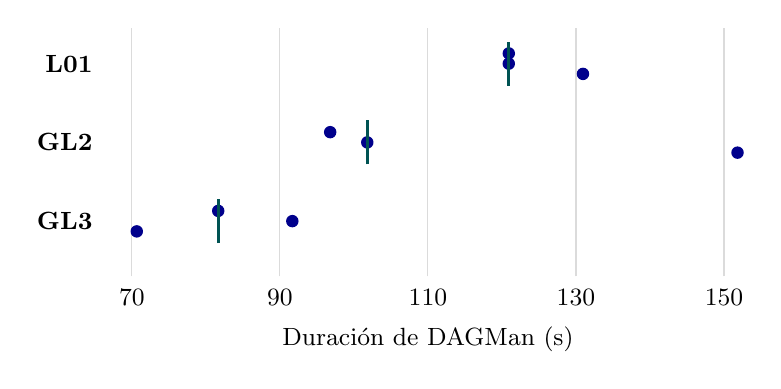
\begin{tikzpicture}[x=0.094cm,y=1cm,font=\small]
\foreach \x in {70,90,110,130,150} {
\draw[gray!28] (\x,0.30)--(\x,3.45);
\node[below] at (\x,0.26) {\x};
}
\node at (110,-0.50) {Duración de DAGMan (s)};
\foreach \y/\name in {3/L01,2/GL2,1/GL3} {
\node[left,font=\small\bfseries] at (66,\y) {\name};
}
\foreach \x/\y in {130.947/2.87,120.922/3.00,120.925/3.13,151.830/1.87,101.803/2.00,96.793/2.13,70.658/0.87,91.678/1.00,81.666/1.13} {
\fill[blue!55!black] (\x,\y) circle (2.25pt);
}
\foreach \x/\y in {120.925/3,101.803/2,81.666/1} {
\draw[teal!65!black,very thick] (\x,\y-0.28)--(\x,\y+0.28);
}
\end{tikzpicture}
\par\smallskip\footnotesize Puntos, ejecuciones individuales. Trazo, mediana. La separación vertical dentro de una misma fila facilita distinguir puntos próximos.
\end{figure}

Las medianas de L01 y GL2 fueron 120,925 y 101,803 s. El máximo de GL2, 151,830 s, superó el de L01, 130,947 s. Las tres duraciones de GL3 quedaron por debajo del mínimo de L01.

Para el archivo compartido, las medianas de AC1, AC2 y AC4 fueron 137,194, 126,833 y 105,815 s, a la vez que bajaron los bytes entregados. Los rangos de AC1 y AC2 se solapan. D02 y GD4 conservaron el volumen y sus medianas fueron 130,967 y 100,836 s. Las diferencias de duración describen las configuraciones completas. La agrupación también cambia el número de jobs, por lo que el diseño no aísla el efecto de los bytes.

\subsection{Criterios para recomendar una configuración}
\label{sec:decisiones_a}
La recomendación depende del criterio del usuario. Para reducir bytes científicos se comparan observados bajo trabajo y fronteras equivalentes. Cuando el requerido positivo es común, un DME mayor corresponde a un volumen observado menor. Si la ubicación cambia, el valor de DME se interpreta con los dos volúmenes y el desglose por destino. En ninguna de estas comparaciones el valor de la razón reemplaza la duración registrada.



\subsection{Sobrecosto de instrumentación}
\label{sec:costo_a}
La medición utiliza los planes y registros nativos de Pegasus y HTCondor. La exportación del historial y el cálculo de DME ocurren después del workflow; sus tiempos no estiman el costo de generar registros durante la ejecución. En la campaña, las medianas de exportación y análisis fueron 0,128 y 0,214 s, respectivamente, con el ejecutable de entonces. No se suman como mediana conjunta ni se atribuyen al código actual. El costo de captura nativa no quedó aislado y limita el cumplimiento de OE4. Los registros individuales se conservan en los materiales.



\subsection{Alcance de la reproducción}
La coincidencia entre repeticiones demuestra consistencia bajo las condiciones ensayadas. Los materiales permiten recalcular los resúmenes del bloque A a partir de datos procesados y ejecutar \Analyzer{} sobre cinco casos históricos portables. Reauditar las 45 ejecuciones desde sus fuentes requiere las cápsulas administrativas. Repetir la medición temporal exige además los ejecutables, sus parámetros y una configuración comparable del entorno.

La validación histórica usa flujos sintéticos pequeños bajo CondorIO; la nueva campaña añade contrastes prospectivos de agrupación y retorno, incluidos dos operadores de Montage. El contraste libre cubre solo el pipeline; la campaña prospectiva mantiene ubicación fija. Otros tamaños o mecanismos requieren contrastes propios. El costo de exportación y análisis se delimita en la sección~\ref{sec:costo_a}.
